\documentclass[11pt,a4paper]{article}
\usepackage[utf8]{inputenc}
\usepackage[T1]{fontenc}
\usepackage{geometry}
\usepackage{graphicx}
\usepackage{amsmath,amssymb,amsfonts}
\usepackage{xcolor}
\usepackage{hyperref}
\usepackage{booktabs}
\usepackage{enumitem}
\usepackage{fancyhdr}
\usepackage{titlesec}
\usepackage{url}
\usepackage{float}
\usepackage{tikz}
\usetikzlibrary{shapes,arrows,positioning}

% Page setup
\geometry{margin=1in}
\pagestyle{fancy}
\fancyhf{}
\fancyhead[L]{\leftmark}
\fancyhead[R]{\thepage}
\fancyfoot[C]{Global Wellness Assistant - Product Documentation}

% Title formatting
\titleformat{\section}{\Large\bfseries}{\thesection}{1em}{}
\titleformat{\subsection}{\large\bfseries}{\thesubsection}{1em}{}
\titleformat{\subsubsection}{\normalsize\bfseries}{\thesubsubsection}{1em}{}

% Colors
\definecolor{primaryblue}{RGB}{13,110,253}
\definecolor{secondaryblue}{RGB}{0,123,255}

% Hyperref setup
\hypersetup{
    colorlinks=true,
    linkcolor=primaryblue,
    filecolor=magenta,
    urlcolor=secondaryblue,
    pdftitle={Global Wellness Assistant - Product Documentation},
    pdfauthor={Global Wellness Team},
    pdfsubject={Health Chatbot System - Product Features}
}

\begin{document}

% Title Page
\begin{titlepage}
\centering
\vspace*{2cm}
{\Huge\bfseries Global Wellness Assistant}\\[0.5cm]
{\Large A Multilingual Health Chatbot System}\\[0.5cm]
{\large Product Documentation \& Feature Guide}\\[2cm]

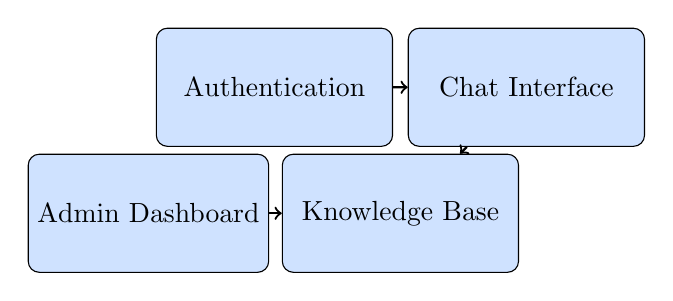
\begin{tikzpicture}[scale=0.8]
    \node[draw, rounded corners, fill=primaryblue!20, minimum width=3cm, minimum height=1.5cm] (auth) at (0,2) {Authentication};
    \node[draw, rounded corners, fill=primaryblue!20, minimum width=3cm, minimum height=1.5cm] (chat) at (4,2) {Chat Interface};
    \node[draw, rounded corners, fill=primaryblue!20, minimum width=3cm, minimum height=1.5cm] (kb) at (2,0) {Knowledge Base};
    \node[draw, rounded corners, fill=primaryblue!20, minimum width=3cm, minimum height=1.5cm] (admin) at (-2,0) {Admin Dashboard};
    \draw[->, thick] (auth) -- (chat);
    \draw[->, thick] (chat) -- (kb);
    \draw[->, thick] (admin) -- (kb);
\end{tikzpicture}

\vspace{2cm}

\begin{minipage}{0.8\textwidth}
\centering
{\large
Global Wellness Team\\
Health Technology Division\\
\vspace{1cm}
Version 1.0\\
November 2024
}
\end{minipage}

\vfill
\end{titlepage}

% Table of Contents
\newpage
\tableofcontents
\newpage

% Abstract
\section*{Executive Summary}
\addcontentsline{toc}{section}{Executive Summary}

The Global Wellness Assistant is a comprehensive, multilingual health chatbot system designed to provide accessible health information and wellness guidance to users worldwide. Built with modern web technologies and advanced conversational AI, the system offers a seamless, secure, and user-friendly experience for health-related queries.

The platform supports multiple languages, with full English and Hindi support, making health information accessible to diverse user populations. The system includes robust user authentication, intelligent symptom recognition, structured health advice, comprehensive administrative tools, and analytics capabilities.

Key differentiators include multilingual support, secure user management, intelligent conversation handling, structured health knowledge base, and comprehensive administrative oversight. The system is designed for scalability, security, and ease of use, making it suitable for deployment in various healthcare and wellness contexts.

\section{Introduction}

\subsection{About Global Wellness Assistant}

The Global Wellness Assistant is an intelligent health chatbot platform that provides immediate, reliable health information and wellness guidance. The system combines the power of conversational AI with a structured health knowledge base to deliver personalized, multilingual health advice.

The platform is designed to bridge the gap between users seeking health information and professional medical resources, providing immediate guidance while always emphasizing the importance of consulting healthcare professionals for serious concerns.

\subsection{Target Audience}

The Global Wellness Assistant serves multiple user groups:

\begin{itemize}
    \item \textbf{General Users}: Individuals seeking quick health information and wellness tips
    \item \textbf{Healthcare Organizations}: Institutions looking to provide 24/7 health information services
    \item \textbf{Administrators}: System managers who need to monitor, manage, and improve the platform
    \item \textbf{Multilingual Communities}: Users who prefer health information in their native language
\end{itemize}

\subsection{Key Benefits}

\begin{itemize}
    \item \textbf{24/7 Availability}: Round-the-clock access to health information
    \item \textbf{Multilingual Support}: Full English and Hindi language support
    \item \textbf{Secure Platform}: Industry-standard authentication and data protection
    \item \textbf{Intelligent Responses}: AI-powered understanding of user queries
    \item \textbf{Structured Information}: Well-organized health advice with clear guidelines
    \item \textbf{User Feedback}: Continuous improvement through user ratings and comments
    \item \textbf{Administrative Control}: Comprehensive tools for system management
\end{itemize}

\section{Product Features Overview}

\subsection{Module 1: User Authentication \& Profile Management}

\subsubsection{User Registration}

Users can create accounts with a simple registration process that includes:
\begin{itemize}
    \item Email-based registration with validation
    \item Secure password creation with strength requirements
    \item Profile information including name and age group
    \item Language preference selection (English or Hindi)
    \item Instant account activation upon successful registration
\end{itemize}

\subsubsection{Secure Authentication}

The platform provides robust authentication features:
\begin{itemize}
    \item Secure login with email and password
    \item Token-based session management
    \item Automatic session expiration for security
    \item Secure logout functionality
    \item Password protection with industry-standard hashing
\end{itemize}

\subsubsection{Profile Management}

Users have full control over their profiles:
\begin{itemize}
    \item View and update personal information
    \item Change language preferences at any time
    \item Update age group for personalized recommendations
    \item Modify account details securely
    \item Profile information synced across all sessions
\end{itemize}

\subsubsection{Language Preferences}

The system supports comprehensive language management:
\begin{itemize}
    \item Choose between English and Hindi
    \item Language preference affects all system interactions
    \item Chat responses automatically in preferred language
    \item Profile interface adapts to language selection
    \item Seamless language switching without data loss
\end{itemize}

\subsection{Module 2: Conversational AI Core}

\subsubsection{Natural Language Understanding}

The chatbot understands health-related queries in natural language:
\begin{itemize}
    \item Recognizes symptom descriptions in plain language
    \item Understands first aid questions
    \item Processes wellness tip requests
    \item Handles greetings and conversational flow
    \item Supports both English and Hindi input
\end{itemize}

\subsubsection{Intelligent Response Generation}

The system provides contextually appropriate responses:
\begin{itemize}
    \item Symptom-specific advice based on user queries
    \item First aid guidance for common injuries
    \item Wellness tips for healthy living
    \item Personalized responses based on user profile
    \item Clear, structured information presentation
\end{itemize}

\subsubsection{Conversation Management}

Advanced conversation handling capabilities:
\begin{itemize}
    \item Multi-turn conversation support
    \item Context awareness across conversation
    \item Session management for conversation continuity
    \item Graceful handling of unclear queries
    \item Fallback responses when information is unavailable
\end{itemize}

\subsubsection{Real-time Chat Interface}

A modern, responsive chat interface provides:
\begin{itemize}
    \item Instant message delivery
    \item Real-time response display
    \item Clean, user-friendly design
    \item Mobile-responsive layout
    \item Smooth conversation flow
\end{itemize}

\subsection{Module 3: Health Knowledge Base \& Multilingual Support}

\subsubsection{Comprehensive Health Information}

The knowledge base contains structured information for:
\begin{itemize}
    \item Common symptoms (headache, fever, cold, sore throat, cough, etc.)
    \item First aid scenarios (burns, cuts, muscle pain)
    \item Wellness tips and healthy living advice
    \item Red flag warnings for serious conditions
    \item Self-care recommendations
\end{itemize}

\subsubsection{Structured Advice Format}

Each health topic provides:
\begin{itemize}
    \item \textbf{Self-Care Tips}: Practical steps users can take at home
    \item \textbf{Red Flags}: Warning signs requiring immediate medical attention
    \item \textbf{Disclaimers}: Clear statements about the informational nature of advice
    \item \textbf{Common Causes}: Understanding of what might cause the condition
\end{itemize}

\subsubsection{Multilingual Content}

Full language support includes:
\begin{itemize}
    \item Complete English content for all health topics
    \item Complete Hindi translations for all entries
    \item Culturally appropriate language and phrasing
    \item Consistent terminology across languages
    \item Native language support for medical terms
\end{itemize}

\subsubsection{Intelligent Symptom Recognition}

The system recognizes symptoms in multiple ways:
\begin{itemize}
    \item Natural language symptom descriptions
    \item Multiple phrasings and variations
    \item Support for both English and Hindi symptom names
    \item Context-aware symptom identification
    \item Automatic mapping to knowledge base entries
\end{itemize}

\subsubsection{Language-Aware Responses}

Responses automatically adapt to user preferences:
\begin{itemize}
    \item Greetings in user's preferred language
    \item Health advice in selected language
    \item Interface elements in appropriate language
    \item Seamless language switching
    \item Consistent multilingual experience
\end{itemize}

\subsection{Module 4: Admin Dashboard \& Analytics}

\subsubsection{Administrative Dashboard}

A comprehensive dashboard provides system overview:
\begin{itemize}
    \item Real-time system statistics
    \item Visual analytics and charts
    \item Quick access to management tools
    \item System health indicators
    \item Recent activity summaries
\end{itemize}

\subsubsection{Knowledge Base Management}

Administrators can manage health content:
\begin{itemize}
    \item View all knowledge base entries
    \item Create new health topics
    \item Edit existing entries
    \item Delete outdated information
    \item Manage multilingual content
    \item Automatic backup before changes
\end{itemize}

\subsubsection{User Feedback Review}

Comprehensive feedback management:
\begin{itemize}
    \item View all user ratings and comments
    \item Identify areas for improvement
    \item Track user satisfaction trends
    \item Review detailed feedback comments
    \item Analyze feedback patterns
\end{itemize}

\subsubsection{Conversation Analytics}

Detailed analytics and insights:
\begin{itemize}
    \item Total conversation count
    \item Conversation volume over time
    \item Most frequently mentioned symptoms
    \item User engagement metrics
    \item Response quality indicators
    \item System usage patterns
\end{itemize}

\subsubsection{Visual Analytics}

Interactive charts and visualizations:
\begin{itemize}
    \item Line charts for conversation trends
    \item Bar charts for symptom frequency
    \item Time-series analysis
    \item Comparative statistics
    \item Export capabilities for reports
\end{itemize}

\subsubsection{Access Control}

Secure administrative access:
\begin{itemize}
    \item Role-based access control
    \item Admin-only route protection
    \item Secure authentication required
    \item Audit trail for administrative actions
    \item Granular permission management
\end{itemize}

\section{User Experience}

\subsection{Getting Started}

\subsubsection{Registration Process}

New users can quickly get started:
\begin{enumerate}
    \item Navigate to the registration page
    \item Enter email address and create password
    \item Provide basic profile information
    \item Select preferred language
    \item Complete registration and start using the system
\end{enumerate}

\subsubsection{First Login}

Upon first login, users can:
\begin{itemize}
    \item Access the chat interface immediately
    \item Update profile information
    \item Explore available features
    \item Set language preferences
    \item Begin asking health questions
\end{itemize}

\subsection{Using the Chat Interface}

\subsubsection{Starting a Conversation}

Users can interact with the chatbot by:
\begin{itemize}
    \item Typing questions in natural language
    \item Asking about symptoms or health concerns
    \item Requesting first aid advice
    \item Seeking wellness tips
    \item Using either English or Hindi
\end{itemize}

\subsubsection{Example Interactions}

\textbf{Symptom Query:}
\begin{itemize}
    \item User: "I have a headache, what should I do?"
    \item System provides structured self-care tips and red flag warnings
\end{itemize}

\textbf{First Aid Query:}
\begin{itemize}
    \item User: "What should I do for a burn?"
    \item System provides step-by-step first aid guidance
\end{itemize}

\textbf{Wellness Query:}
\begin{itemize}
    \item User: "How can I sleep better?"
    \item System provides wellness tips and healthy living advice
\end{itemize}

\subsubsection{Providing Feedback}

After each bot response, users can:
\begin{itemize}
    \item Rate the response (1-5 stars)
    \item Add optional comments
    \item Submit feedback instantly
    \item Help improve the system
\end{itemize}

\subsection{Profile Management}

\subsubsection{Viewing Profile}

Users can view their profile information:
\begin{itemize}
    \item Personal details
    \item Account creation date
    \item Language preferences
    \item Age group information
\end{itemize}

\subsubsection{Updating Profile}

Profile updates are simple:
\begin{itemize}
    \item Edit name and age group
    \item Change language preference
    \item Updates apply immediately
    \item Changes reflected in all system interactions
\end{itemize}

\section{Administrative Features}

\subsection{Dashboard Overview}

Administrators access a comprehensive dashboard showing:
\begin{itemize}
    \item \textbf{Total Conversations}: Overall system usage
    \item \textbf{Total Feedback}: User engagement metrics
    \item \textbf{Average Rating}: User satisfaction score
    \item \textbf{Distinct Symptoms}: Variety of health topics discussed
\end{itemize}

\subsection{Knowledge Base Management}

\subsubsection{Content Management}

Administrators can manage health content through an intuitive interface:
\begin{itemize}
    \item \textbf{View All Entries}: Browse complete knowledge base
    \item \textbf{Create New Topics}: Add new health information
    \item \textbf{Edit Existing Content}: Update and improve entries
    \item \textbf{Delete Outdated Information}: Remove obsolete content
    \item \textbf{Multilingual Editing}: Manage both English and Hindi content
\end{itemize}

\subsubsection{Content Structure}

Each knowledge base entry includes:
\begin{itemize}
    \item Category classification (symptom or first aid)
    \item Common causes information
    \item Self-care recommendations
    \item Red flag warnings
    \item Medical disclaimers
    \item Complete Hindi translations
\end{itemize}

\subsection{Feedback Management}

\subsubsection{Reviewing Feedback}

Administrators can review user feedback to:
\begin{itemize}
    \item Understand user satisfaction levels
    \item Identify areas needing improvement
    \item Read detailed user comments
    \item Track feedback trends over time
    \item Make data-driven improvements
\end{itemize}

\subsubsection{Feedback Insights}

The system provides insights into:
\begin{itemize}
    \item Average user ratings
    \item Most common feedback themes
    \item User satisfaction trends
    \item Areas receiving positive feedback
    \item Opportunities for enhancement
\end{itemize}

\subsection{Analytics \& Reporting}

\subsubsection{Conversation Analytics}

Detailed conversation metrics include:
\begin{itemize}
    \item Daily conversation volume
    \item Conversation trends over time
    \item Peak usage periods
    \item User engagement patterns
    \item Response effectiveness metrics
\end{itemize}

\subsubsection{Symptom Analytics}

Health topic insights provide:
\begin{itemize}
    \item Most frequently discussed symptoms
    \item Symptom frequency rankings
    \item Seasonal health trends
    \item Common health concerns
    \item Knowledge base usage patterns
\end{itemize}

\subsubsection{Visual Reports}

Interactive charts display:
\begin{itemize}
    \item Time-series conversation data
    \item Symptom frequency comparisons
    \item Trend analysis
    \item Comparative statistics
    \item Export-ready visualizations
\end{itemize}

\section{System Capabilities}

\subsection{Multilingual Support}

\subsubsection{Language Features}

The system provides comprehensive multilingual capabilities:
\begin{itemize}
    \item Full English and Hindi language support
    \item Automatic language detection from user profile
    \item Language-aware response generation
    \item Seamless language switching
    \item Consistent terminology across languages
\end{itemize}

\subsubsection{Language Coverage}

Both languages support:
\begin{itemize}
    \item Complete user interface
    \item All health knowledge base content
    \item Chatbot responses
    \item System messages and notifications
    \item Administrative interfaces
\end{itemize}

\subsection{Security Features}

\subsubsection{User Data Protection}

The platform implements robust security measures:
\begin{itemize}
    \item Secure password storage with industry-standard hashing
    \item Encrypted authentication tokens
    \item Protected user sessions
    \item Secure data transmission
    \item Privacy-focused design
\end{itemize}

\subsubsection{Access Control}

Comprehensive access management:
\begin{itemize}
    \item Role-based permissions
    \item Admin-only route protection
    \item Secure authentication required
    \item Session expiration
    \item Secure logout functionality
\end{itemize}

\subsection{Reliability Features}

\subsubsection{Error Handling}

The system gracefully handles various scenarios:
\begin{itemize}
    \item Service unavailability
    \item Network connectivity issues
    \item Invalid user inputs
    \item System errors
    \item Graceful degradation
\end{itemize}

\subsubsection{Data Protection}

Comprehensive data safety measures:
\begin{itemize}
    \item Automatic backups before changes
    \item Data integrity checks
    \item Recovery mechanisms
    \item Safe file operations
    \item Transaction management
\end{itemize}

\section{Use Cases}

\subsection{Individual Users}

\subsubsection{Quick Health Information}

Users can quickly access health information for:
\begin{itemize}
    \item Understanding common symptoms
    \item Learning self-care techniques
    \item Getting first aid guidance
    \item Receiving wellness tips
    \item Clarifying health concerns
\end{itemize}

\subsubsection{Multilingual Access}

Users who prefer non-English content can:
\begin{itemize}
    \item Access all information in Hindi
    \item Ask questions in their preferred language
    \item Receive responses in their language
    \item Navigate the interface in their language
    \item Enjoy a fully localized experience
\end{itemize}

\subsection{Healthcare Organizations}

\subsubsection{24/7 Information Service}

Organizations can provide:
\begin{itemize}
    \item Round-the-clock health information access
    \item Consistent, reliable information delivery
    \item Multilingual service capabilities
    \item Reduced support staff workload
    \item Scalable information distribution
\end{itemize}

\subsubsection{Administrative Oversight}

Organizations benefit from:
\begin{itemize}
    \item Comprehensive usage analytics
    \item Content management capabilities
    \item User feedback insights
    \item System monitoring tools
    \item Performance metrics
\end{itemize}

\subsection{System Administrators}

\subsubsection{Content Management}

Administrators can:
\begin{itemize}
    \item Maintain and update health content
    \item Add new health topics
    \item Improve existing information
    \item Manage multilingual content
    \item Ensure information accuracy
\end{itemize}

\subsubsection{System Monitoring}

Administrative tools enable:
\begin{itemize}
    \item Real-time system monitoring
    \item Usage pattern analysis
    \item Performance tracking
    \item User engagement metrics
    \item System health assessment
\end{itemize}

\section{Key Differentiators}

\subsection{Multilingual Excellence}

The Global Wellness Assistant stands out with:
\begin{itemize}
    \item Complete bilingual support (English/Hindi)
    \item Native language symptom recognition
    \item Culturally appropriate responses
    \item Seamless language switching
    \item Consistent multilingual experience
\end{itemize}

\subsection{Intelligent Understanding}

Advanced AI capabilities provide:
\begin{itemize}
    \item Natural language understanding
    \item Context-aware responses
    \item Symptom recognition from descriptions
    \item Multi-turn conversation handling
    \item Intelligent fallback mechanisms
\end{itemize}

\subsection{Comprehensive Health Information}

Structured knowledge base offers:
\begin{itemize}
    \item Well-organized health topics
    \item Clear self-care guidance
    \item Important red flag warnings
    \item Medical disclaimers
    \item Reliable, vetted information
\end{itemize}

\subsection{Administrative Excellence}

Powerful admin tools enable:
\begin{itemize}
    \item Easy content management
    \item Comprehensive analytics
    \item User feedback insights
    \item System monitoring
    \item Data-driven improvements
\end{itemize}

\section{System Requirements}

\subsection{User Requirements}

Users need:
\begin{itemize}
    \item Modern web browser (Chrome, Firefox, Safari, Edge)
    \item Internet connection
    \item JavaScript enabled
    \item No additional software installation
\end{itemize}

\subsection{Platform Requirements}

The system runs on:
\begin{itemize}
    \item Web-based platform (no installation needed)
    \item Responsive design for all devices
    \item Mobile-friendly interface
    \item Cross-platform compatibility
    \item Cloud-ready architecture
\end{itemize}

\section{Privacy \& Security}

\subsection{Data Privacy}

The platform respects user privacy:
\begin{itemize}
    \item Secure data storage
    \item Encrypted communications
    \item Minimal data collection
    \item User control over information
    \item Privacy-focused design
\end{itemize}

\subsection{Security Measures}

Comprehensive security implementation:
\begin{itemize}
    \item Industry-standard authentication
    \item Secure password handling
    \item Protected user sessions
    \item Secure API communications
    \item Regular security updates
\end{itemize}

\section{Medical Disclaimers}

\subsection{Important Notice}

The Global Wellness Assistant provides general wellness information only. It is \textbf{NOT} a substitute for professional medical advice, diagnosis, or treatment.

\subsection{When to Seek Professional Help}

Users should consult healthcare professionals for:
\begin{itemize}
    \item Serious or persistent symptoms
    \item Medical emergencies
    \item Diagnosis and treatment decisions
    \item Medication questions
    \item Any concerning health conditions
\end{itemize}

\subsection{Red Flag Warnings}

The system includes clear warnings for:
\begin{itemize}
    \item Symptoms requiring immediate medical attention
    \item Serious health conditions
    \item Emergency situations
    \item High-risk scenarios
    \item Conditions needing professional evaluation
\end{itemize}

\section{Future Roadmap}

\subsection{Planned Enhancements}

Upcoming features include:
\begin{itemize}
    \item Additional language support
    \item Expanded health knowledge base
    \item Advanced personalization
    \item Integration with health APIs
    \item Mobile applications
    \item Voice interface support
    \item Enhanced analytics
    \item Conversation history
    \item Telemedicine integration
\end{itemize}

\subsection{Continuous Improvement}

The system evolves through:
\begin{itemize}
    \item User feedback integration
    \item Regular content updates
    \item Performance optimizations
    \item Feature enhancements
    \item Security improvements
    \item User experience refinements
\end{itemize}

\section{Support \& Resources}

\subsection{User Support}

Users can access:
\begin{itemize}
    \item In-system help and guidance
    \item Clear interface instructions
    \item Feedback mechanisms
    \item System documentation
    \item Frequently asked questions
\end{itemize}

\subsection{Administrative Resources}

Administrators have access to:
\begin{itemize}
    \item Comprehensive admin dashboard
    \item System documentation
    \item Analytics and reporting tools
    \item Content management guides
    \item Best practices documentation
\end{itemize}

\section{Conclusion}

The Global Wellness Assistant represents a comprehensive solution for delivering accessible, multilingual health information to users worldwide. With its robust authentication system, intelligent conversational AI, structured health knowledge base, and comprehensive administrative tools, the platform provides a complete ecosystem for health information delivery.

The system's multilingual capabilities, security features, and user-friendly design make it suitable for diverse user populations and organizational contexts. The comprehensive administrative tools enable effective system management and continuous improvement.

Key strengths include:
\begin{itemize}
    \item Complete multilingual support
    \item Secure and reliable platform
    \item Intelligent conversation handling
    \item Comprehensive health information
    \item Powerful administrative tools
    \item User-focused design
    \item Scalable architecture
\end{itemize}

The Global Wellness Assistant is positioned to serve as a valuable tool in making health information more accessible, supporting users in their wellness journeys while always emphasizing the importance of professional medical care when needed.

\section*{Contact Information}

For inquiries, support, or additional information about the Global Wellness Assistant, please contact:

\begin{itemize}
    \item \textbf{Project Team}: Global Wellness Team
    \item \textbf{Division}: Health Technology Division
    \item \textbf{Version}: 1.0
    \item \textbf{Last Updated}: November 2024
\end{itemize}

\end{document}

